\documentclass[12pt]{article}
\usepackage{amsthm,amssymb,amsfonts,amsmath,amstext,systeme}
\usepackage{graphicx,float}
\usepackage{tabularx}

\marginparwidth 0pt
\oddsidemargin -1.2 truecm
\evensidemargin  0pt 
\marginparsep 0pt
\topmargin -2.2truecm
\linespread{1}
\textheight 25.8 truecm
\textwidth 18.5 truecm
\newenvironment{remark}{\noindent{\bf Remark }}{\vspace{0mm}}
\newenvironment{remarks}{\noindent{\bf Remarks }}{\vspace{0mm}}
\newenvironment{question}{\noindent{\bf Question }}{\vspace{0mm}}
\newenvironment{questions}{\noindent{\bf Questions }}{\vspace{0mm}}
\newenvironment{note}{\noindent{\bf Note }}{\vspace{0mm}}
\newenvironment{summary}{\noindent{\bf Summary }}{\vspace{0mm}}
\newenvironment{back}{\noindent{\bf Background}}{\vspace{0mm}}
\newenvironment{conclude}{\noindent{\bf Conclusion}}{\vspace{0mm}}
\newenvironment{concludes}{\noindent{\bf Conclusions}}{\vspace{0mm}}
\newenvironment{dill}{\noindent{\bf Description of Dill's model}}{\vspace{0mm}}
\newenvironment{maths}{\noindent{\bf Mathematics needed}}{\vspace{0mm}}
\newenvironment{inst}{\noindent{\bf Instructions}}{\vspace{0mm}}
\newenvironment{notes}{\noindent{\bf Notes }}{\vspace{0mm}}
\newenvironment{theorem}{\noindent{\bf Theorem }}{\vspace{0mm}}
\newenvironment{example}{\noindent{\bf Example }}{\vspace{0mm}}
\newenvironment{examples}{\noindent{\bf Examples }}{\vspace{0mm}}
\newenvironment{topics}{\noindent{\bf Topics}}{\vspace{0mm}}
\newenvironment{outcomes}{\noindent{\bf Expected Learning Outcomes}}{\vspace{0mm}}
\newenvironment{lemma}{\noindent{\bf Lemma }}{\vspace{0mm}}
\newenvironment{solution}{\noindent{\it Solution}}{\vspace{2mm}}
\newcommand{\ds}{\displaystyle}
\newcommand{\un}{\underline}
\newcommand{\bs}{\boldsymbol}

\begin{document}

\baselineskip 18 pt
\begin{center}
	{\large \bf HKDSE MATH CORE 2015 Past Paper I}\\
	\vspace{2 mm}

\end{center}
\vspace{0.05cm}

\begin{enumerate}
	\item \textbf{HKDSE MATH CORE 2015 Past Paper I Q1}\\
	Simplify $\dfrac{m^9}{(m^3n^{-7})^5}$ and express your answer with positive indices. \\(3 marks)	
	
	\item \textbf{HKDSE MATH CORE 2015 Past Paper I Q2}\\
	Make $b$ the subject of the formula $\dfrac{4a+5b-7}{b} = 8$. \\(3 marks)

	\item \textbf{HKDSE MATH CORE 2015 Past Paper I Q3}
	Bag A contains four cards numbered 1, 3, 5 and 7 respectively while bag B contains five cards numbered 2, 4, 6, 8 and 10 respectively. If one card is randomly drawn from each bag, find the probability that the sum of the two numbers drawn is less than 9. \\(3 marks)

	\item \textbf{HKDSE MATH CORE 2015 Past Paper I Q4}\\
	Factorize
	\begin{enumerate}
		\item[(a)] $x^3 + x^2y -7x^2$,
		\item[(b)] $x^3 + x^2y -7x^2 -x -y +7$.
	\end{enumerate}
	(4 marks)

	\item \textbf{HKDSE MATH CORE 2015 Past Paper I Q5}\\
	Consider the formula $2(3m +n) = m + 7$.
	\begin{enumerate}
		\item[(a)] Find the range of values of x which satisfy both $\dfrac{7 - 3x}{5} \leq 2(x+2)$ and $4x - 13>0$.
		\item[(b)] Write down the least integer which satisfies both inequalities in (a).	
	\end{enumerate}
	(4 marks)
   
	\item \textbf{HKDSE MATH CORE 2015 Past Paper I Q6}\\
	The cost of a book is \$250. The book is now sold and the percentage profit is 20\%.
	\begin{enumerate}
		\item[(a)] Find the selling price of the book.
		\item[(b)] If the book is sold at a discount of 25\% on its marked price, find the marked price of the book.
	\end{enumerate}
	(4 marks)

	\item \textbf{HKDSE MATH CORE 2015 Past Paper I Q7}\\
	The number of apples owned by Ada is 4 times that owned by Billy. If Ada gives 12 of her apples to Billy, they will have the same number of apples. Find the total number of apples owned by Ada and Billy. \\(4 marks)
	
	\item \textbf{HKDSE MATH CORE 2015 Past Paper I Q8}\\
	In Figure 1, $ABCD$ is a circle. $E$ is a point lying on $AC$ such that $BC = CE$. It is given that $AB = AD$. $\angle ADB = 58^\circ$ and $\angle CBD = 25^\circ$.
	\begin{figure}[H]
		\centering
		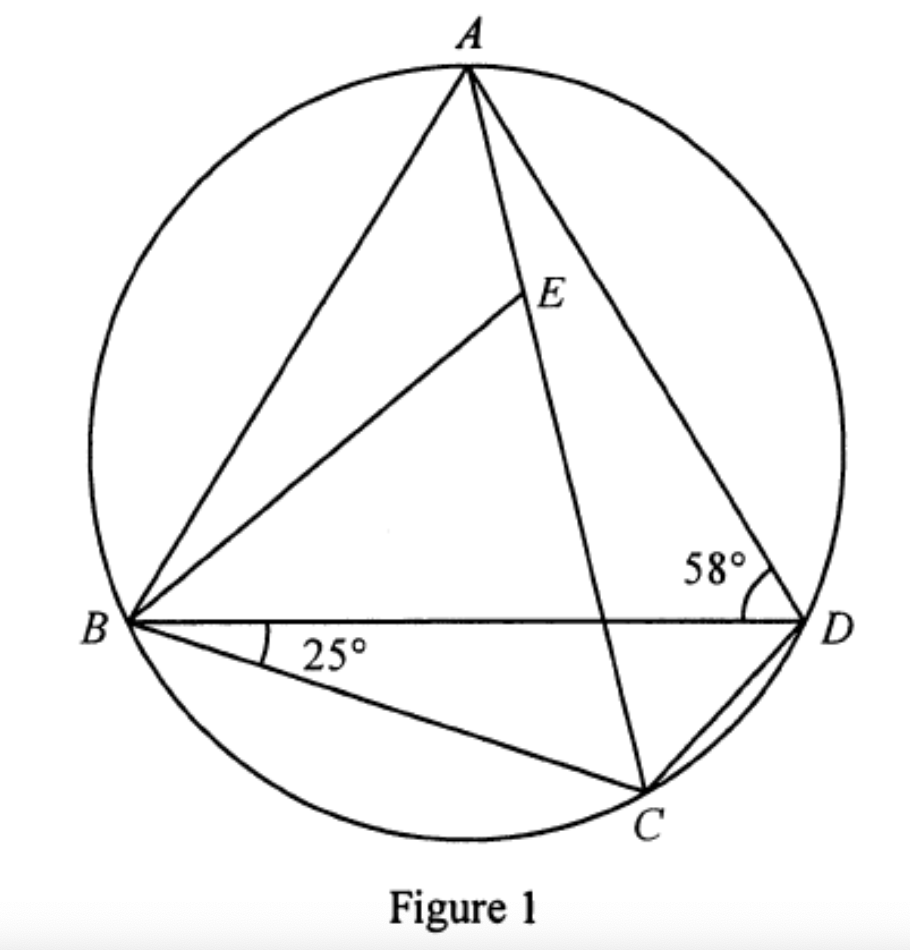
\includegraphics[width = .3\linewidth]{2015Figure1.1}
	\end{figure}
	Find $\angle BDC$ and $\angle ABE$. \\(5 marks)
	
	\item \textbf{HKDSE MATH CORE 2015 Past Paper I Q9}\\
	The radius and the area of a sector are 12 cm and $30\pi$ cm$^2$ respectively.
	\begin{enumerate}
		\item[(a)] Find the angle of the sector.
		\item[(b)] Express the perimeter of the sector in terms of $\pi$.
	\end{enumerate}
	(5 marks)

	\item \textbf{HKDSE MATH CORE 2015 Past Paper I Q10}\\
	When Susan sells n handbags in a month, her income in that month is $\$S$. It is given that $S$ is a sum of two parts, one part is a constant and the other part varies as $n$. When $n$ = 10, $S$ = 10 600; when $n = 6$, $S$ = 9 000.
	\begin{enumerate}
		\item[(a)] When Susan sells 20 handbags in a month, find her income in that month. \\(4 marks)
		\item[(b)] Is it possible that when Susan sells a certain number of handbags in a month, her income in that month is \$18 000? Explain your answer. \\(2 marks)
	\end{enumerate}

	\item \textbf{HKDSE MATH CORE 2015 Past Paper I Q11}\\
	Let $f(x) = (x - 2)^2(x+h)+k$, where $h$ and $k$ are constants. When  $f(x)$ is divided by $x - 2$, the remainder is 5. It is given that  $f(x)$ is divisible by $x - 3$.
	\begin{enumerate}
		\item[(a)] Find $h$ and $k$. \\(3 marks)
		\item[(b)] Someone claims that all the roots of the equation  $f(x) = 0$ are integers. Do you agree? Explain your answer. \\(3 marks)
	\end{enumerate}

	\item \textbf{HKDSE MATH CORE 2015 Past Paper I Q12}\\
	The stem-and-leaf diagram below shows the distribution of the weights (in kg) of the students in a football club.
	\begin{table}[htbp]
		\centering
		\begin{tabular}{r|l@{\hspace{4 pt}}l@{\hspace{4 pt}}l@{\hspace{4 pt}}l@{\hspace{4 pt}}}
		   Stem (tens) & Leaf (units)     \\
			\hline
			4     & 0 2 3 3 3 3 9\\    
			5     & 1 1 2 2 3 7 9\\    
			6     & 3 5 8 9\\    
			7     & 8 9\\    
		\end{tabular}
		% \label{tab:addlabel}
	\end{table}
	\begin{enumerate}
		\item[(a)] Find the mean, the median and the range of the above distribution. \\(3 marks)
		\item[(b)] Two more students now join the club. It is found that both the mean and the range of the distribution of the weights are increased by 1 kg. Find the weight of each of these two students. \\(4 marks)
	\end{enumerate}

	\item \textbf{HKDSE MATH CORE 2015 Past Paper I Q13}\\
	In Figure 2, $ABCD$ is a square. $E$ and $F$ are points lying on $BC$ and $CD$ respectively such that $AE = BF$. $AE$ and $BF$ intersect at $G$.
	\begin{figure}[H]
		\centering
		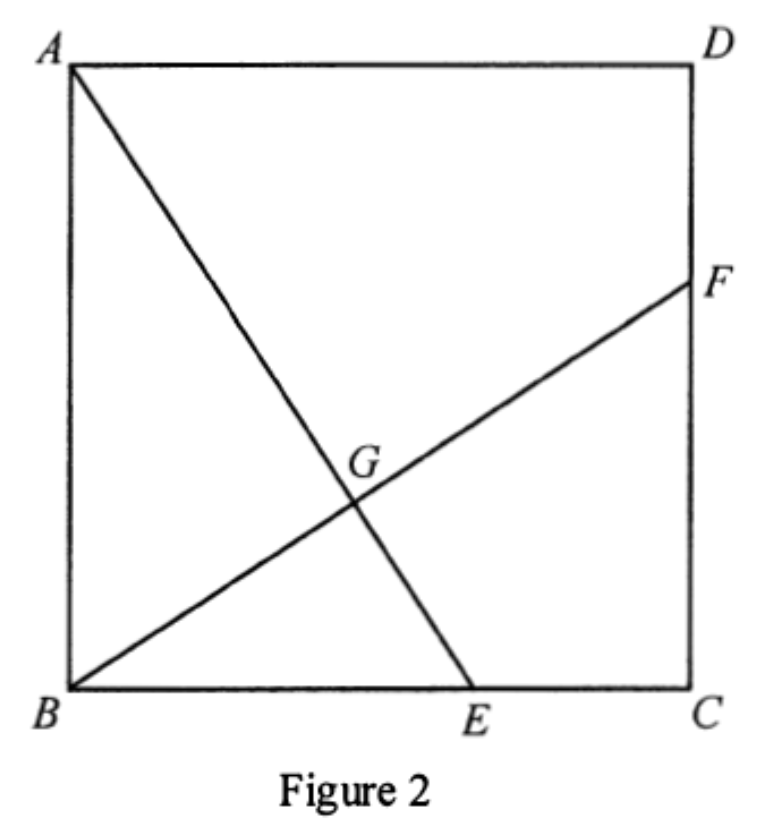
\includegraphics[width = .3\linewidth]{2015Figure1.2}
	\end{figure}
	\begin{enumerate}
		\item[(a)] Prove that $\triangle ABE \cong \triangle BCF$. \\(2 marks)
		\item[(b)] Is $\triangle BGE$ a right-angled triangle? Explain your answer. \\(3 marks)
		\item[(c)] If $CF = 15$ cm and $EG = 9$ cm, find $BG$. \\(2 marks)
	\end{enumerate}

	\item \textbf{HKDSE MATH CORE 2015 Past Paper I Q14}\\
	The coordinates of the points $P$ and $Q$ are $(4, -1)$ and $(-14, 23)$ respectively.
	\begin{enumerate}
		\item[(a)] Let $L$ be the perpendicular bisector of $PQ$.
		\begin{enumerate}
			\item[(i)] Find the equation of $L$.
			\item[(ii)] Suppose $G$ is a point lying on $L$. Denote the $x$-coordinate of $G$ by $h$. Let $C$ be the circle which is centred at $G$ and passes through $P$ and $Q$. Prove that the equation of $C$ is $2x^2 + 2y^2 -4hx -(3h+59)y + 13h - 93 = 0$.
		\end{enumerate}
		(6 marks)
		\item[(b)] The coordinates of the point $R$ are $(26, 43)$. Using (a)(ii), or otherwise, find the diameter of the circle which passes through $P$, $Q$ and $R$. \\(3 marks)
	\end{enumerate}

	\item \textbf{HKDSE MATH CORE 2015 Past Paper I Q15}\\
	The table below shows the means and the standard deviations of the scores of a large group of students in a Mathematics examination and a Science examination:
	$$\begin{array}{|c|c|c|}
		\hline
		\text{Examination} & \text{Mean} & \text{Standard deviation} \\
		\hline
		\text{Mathematics} & \text{66 marks} & \text{12 marks} \\
		\hline		
		\text{Science} & \text{52 marks} & \text{10 marks} \\
		\hline
	\end{array}$$
	The standard score of David in the Mathematics examination is $-0.5$.
	\begin{enumerate}
		\item[(a)] Find the score of David in the Mathematics examination. \\(2 marks)
		\item[(b)] Assume that the scores in each of the above examinations are normally distributed. David gets 49 marks in the Science examination. He claims that relative to other students, he performed better in the Science examination than in the Mathematics examination. Is the claim correct? Explain your answer. \\(2 marks)
	\end{enumerate}

	\item \textbf{HKDSE MATH CORE 2015 Past Paper I Q16}\\
	A box contains 5 red bowls, 6 yellow bowls and 3 white bowls. If 4 bowls are randomly drawn from the box at the same time,
	\begin{enumerate}
		\item[(a)] find the probability that exactly 2 red bowls are drawn; \\(2 marks)
		\item[(b)] find the probability that at least 2 red bowls are drawn. \\(2 marks)
	\end{enumerate}

	\item \textbf{HKDSE MATH CORE 2015 Past Paper I Q17}\\
	For any positive integer $n$, let $A(n) = 4n - 5$ and $B(n) = 10^{4n-5}$.
	\begin{enumerate}
		\item[(a)] Express $A(1) + A(2) + A(3) + \cdots + A(n)$ in terms of $n$. \\(2 marks)
		\item[(b)] Find the greatest value of n such that $\log{(B(1)B(2)B(3)\cdots B(n))}\leq 8000$. \\(3 marks)
	\end{enumerate}

	\item \textbf{HKDSE MATH CORE 2015 Past Paper I Q18}\\
	Let $f(x) = 2x^2 -4kx + 3k^2 + 5$, where $k$ is a real constant.
	\begin{enumerate}
		\item[(a)] Does the graph of $y = f(x)$ cut the $x$-axis? Explain your answer. \\(2 marks)
		\item[(b)] Using the method of completing the square, express, in terms of $k$, the coordinates of the vertex of the graph of $y = f(x)$. \\(3 marks)
		\item[(c)] In the same rectangular coordinate plane, let $S$ and $T$ be moving points on the graph of $y = f(x)$ and the graph of $y = 2 - f(x)$ respectively. Denote the origin by $O$. Someone claims that when $S$ and $T$ are nearest to each other, the circumcentre of $\triangle OST$ lies on the $x$-axis. Is the claim correct? Explain your answer. \\(4 marks)
	\end{enumerate}

	\item \textbf{HKDSE MATH CORE 2015 Past Paper I Q19}\\
	In Figure 3(a), $ABCDB'$ is a pentagonal paper card. It is given that $AB = AB' = 40$ cm, $BC = B'D = 24$ cm and $\angle ABC = \angle AB'D = 80^\circ$.
	\begin{figure}[H]
		\centering
		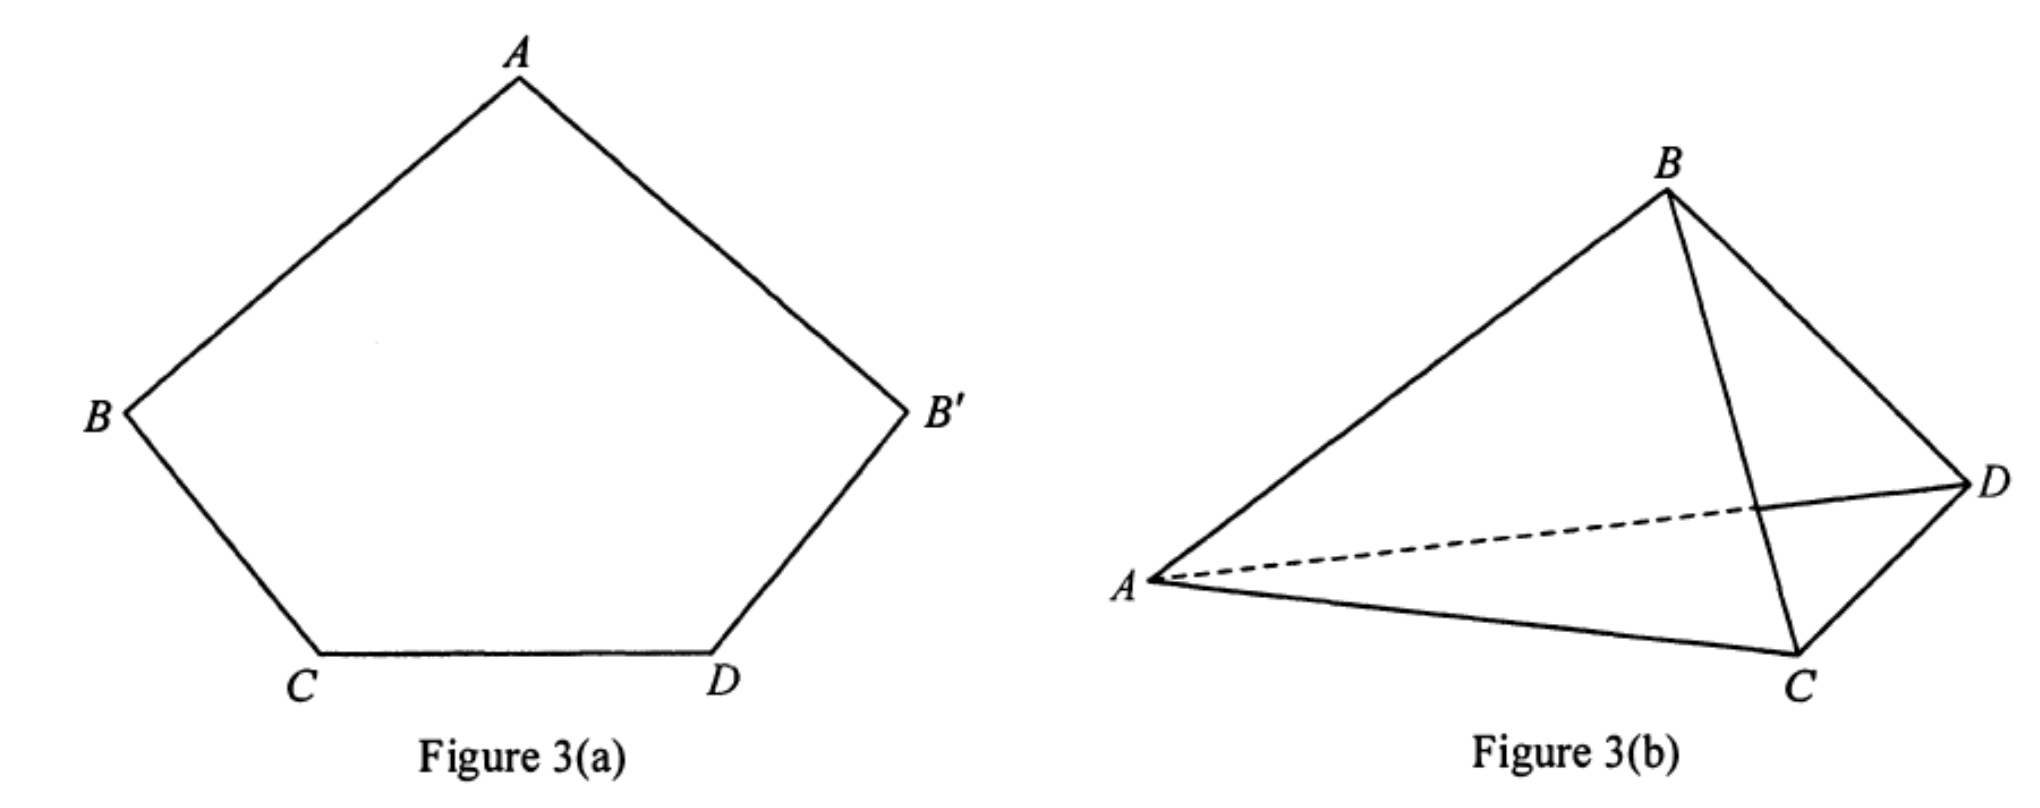
\includegraphics[width = .3\linewidth]{2015Figure1.3}
	\end{figure}
	\begin{enumerate}
		\item[(a)] Suppose that $105^\circ \leq \angle BCD \leq 145^\circ$.
		\begin{enumerate}
			\item[(i)] Find the distance between $A$ and $C$.
			\item[(ii)] Find $\angle ACB$.
			\item[(iii)] Describe how the area of the paper card varies when $\angle BCD$ increases from $105^\circ$ to $145^\circ$. Explain your answer.
		\end{enumerate}
		(7 marks)
		\item[(b)] Suppose that $\angle BCD = 132^\circ$. The paper card in Figure 3(a) is folded along $AC$ and $AD$ such that $AB$ and $AB'$ join together to form a pyramid $ABCD$ as shown in Figure 3(b). Find the volume of the pyramid $ABCD$. \\(6 marks)
	\end{enumerate}
\end{enumerate}


\end{document}